\chapter{Excavator Setup}\label{ch:excavatorSetup}

\begin{figure}[ht]
    \centering
    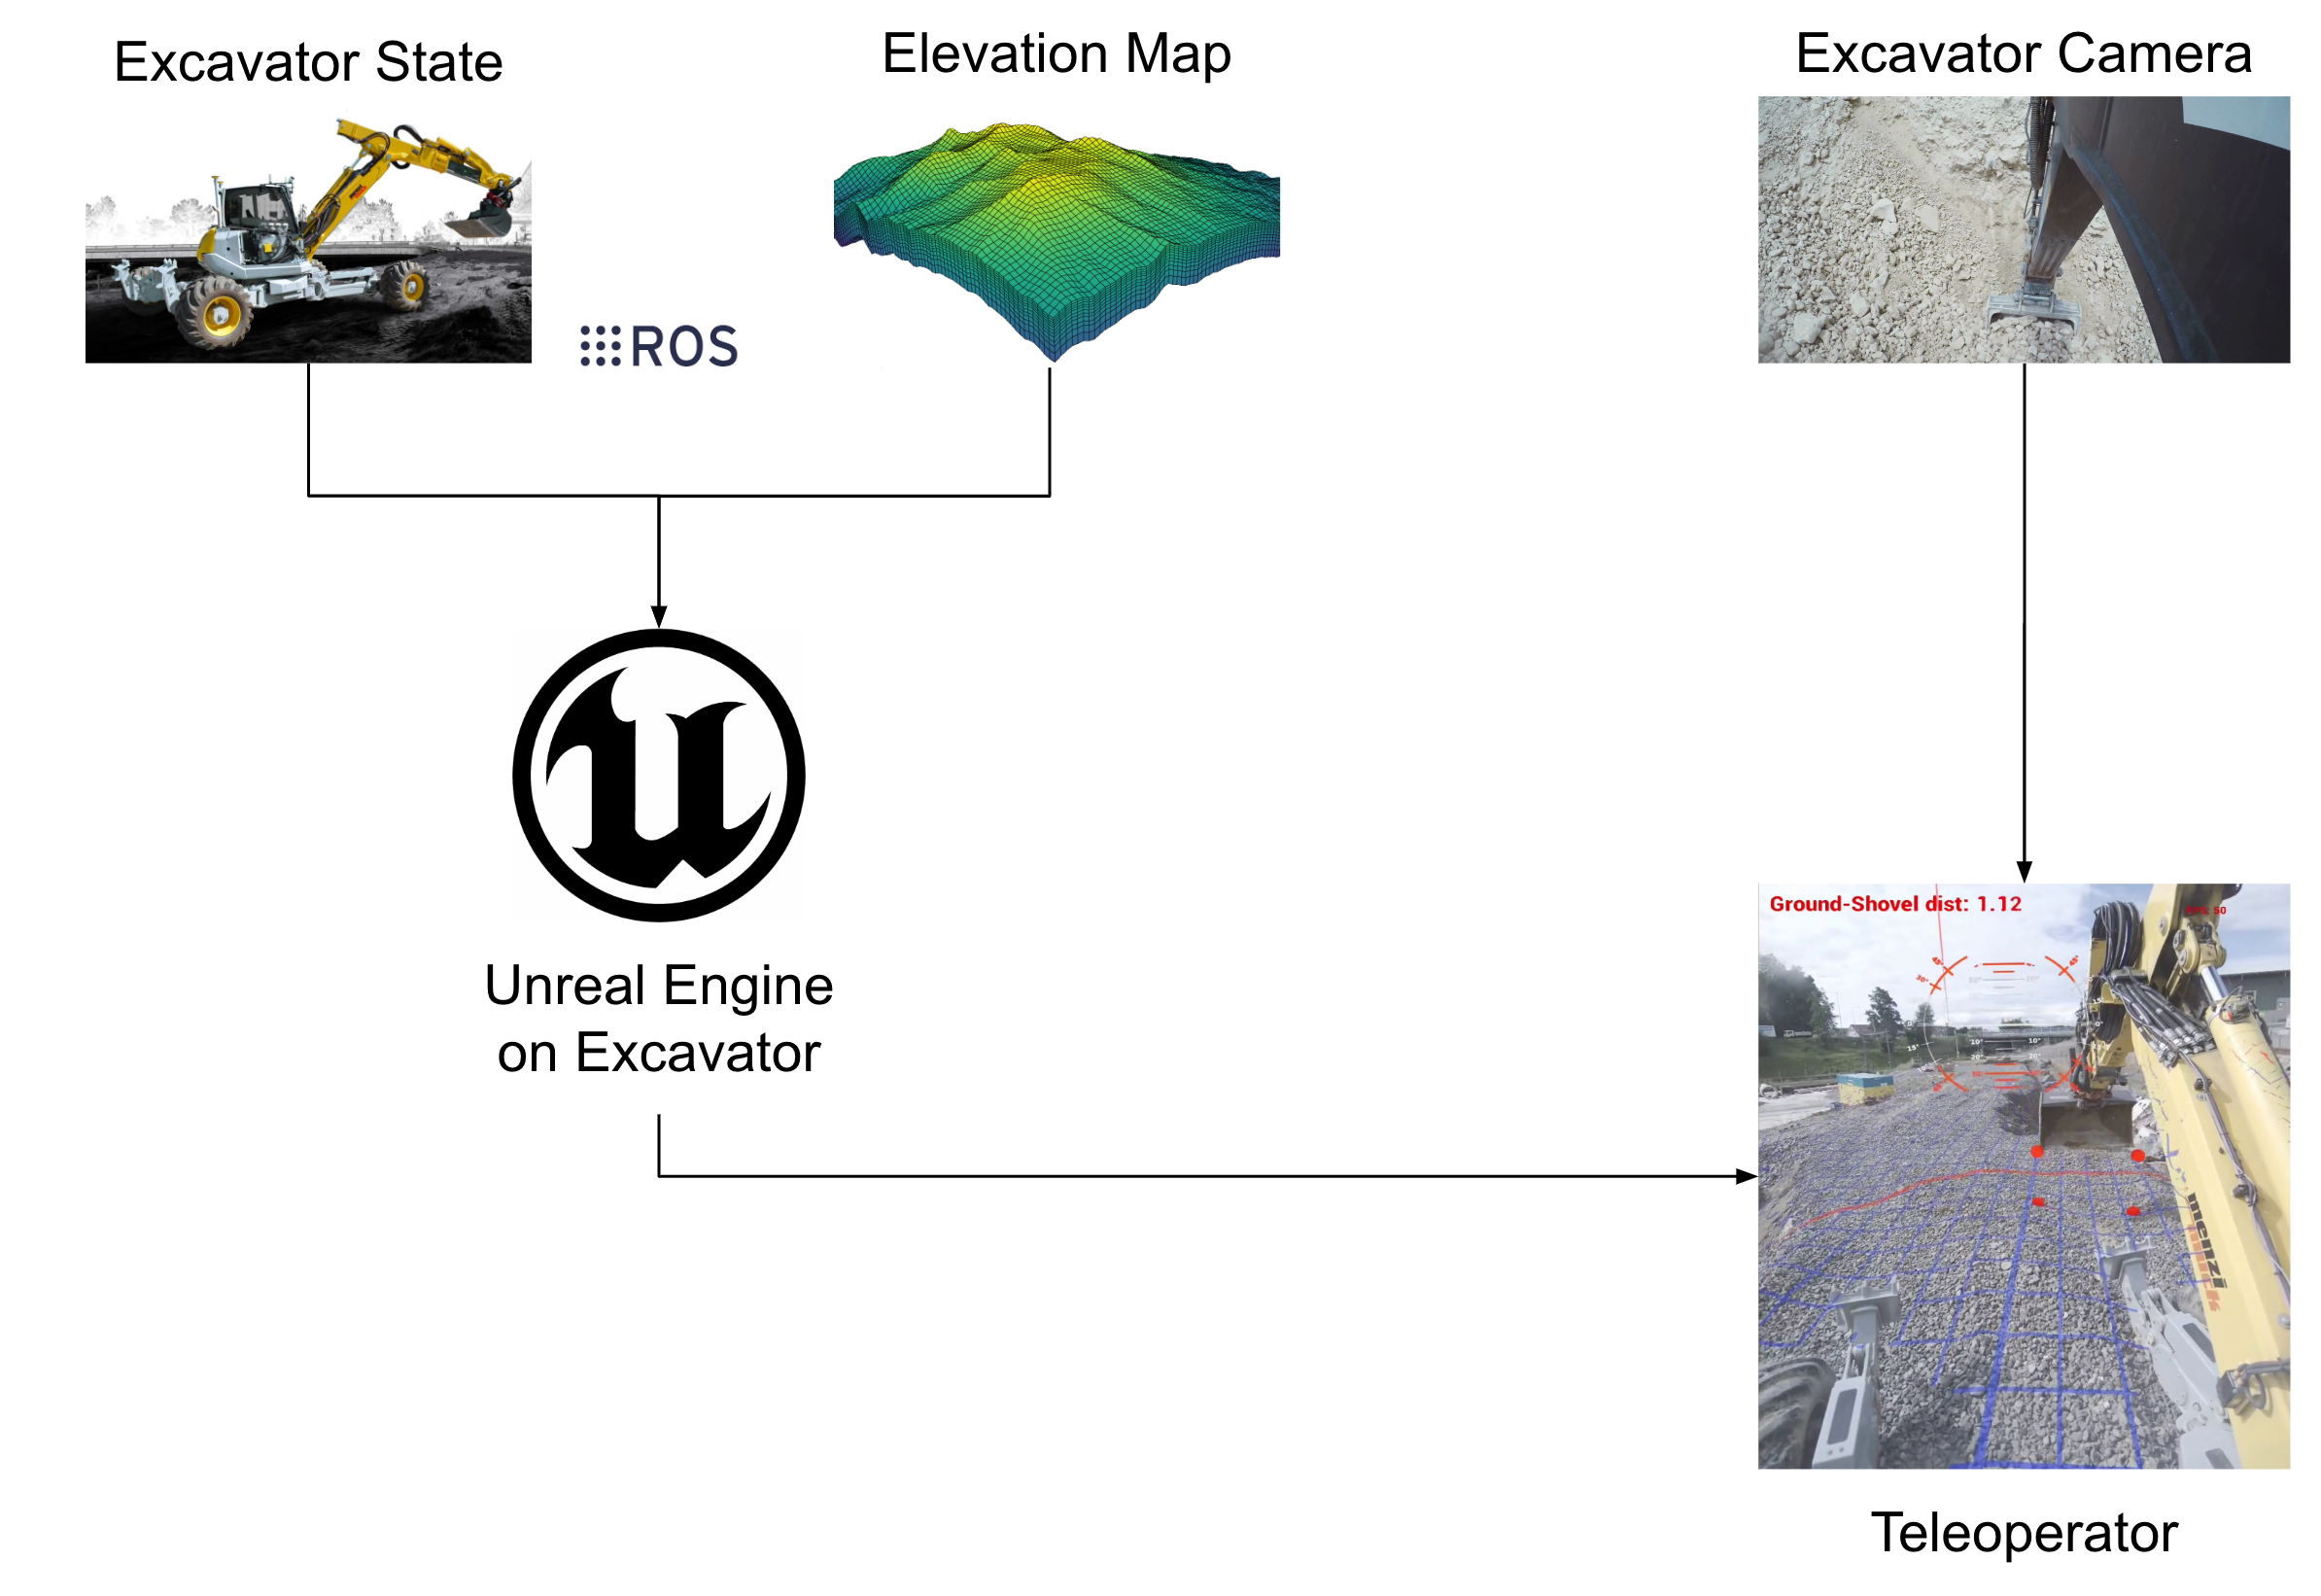
\includegraphics[scale = 0.3]{images/excavator/excavator_setup.png}
    \caption{High level excavator setup prior to this project}
    \label{fig:ex_setup}
\end{figure}

The excavator has an Unreal Engine instance running on it. In the UE instance there is a model of the excavator which is updated continuously using a built in ROS subscriber in UE. 

Another crucial input to the excavator is an elevation map which is generated from the visual input of the environment.

Through the current state of the excavator at any time it is possible to calculate the parts in the camera input image which are occluded by the excavator. This feature allows for the creation of a mask to cut the excavator out of the elevation map projection.

In the end the Unreal Engine instance outputs this tailored elevation map projection which can be applied on top of the input image which is fed to the teleoperator.

In the handheld setup we can make use of this pipeline to fullfill our specific requirements and down the road enable high level remote control inputs.
